\section{Results}
\label{sec:results}

We organize the analysis around six research questions. All metric values are means over 100 SQuAD questions.

\subsection{RQ1: How Do Generation Models Compare?}

Table~\ref{tab:model-comparison} aggregates results across all configurations for each model. For each model, we report the mean and best observed values for key metrics.

\begin{table}[t]
\centering
\caption{Model comparison: mean and (best) across all configurations. Faithfulness (Faith.), nDCG@5, BERTScore F1 (BS-F1), and METEOR are reported.}
\label{tab:model-comparison}
\resizebox{\textwidth}{!}{%
\begin{tabular}{lcccc}
\toprule
\textbf{Model} & \textbf{Faith.} $\uparrow$ & \textbf{nDCG@5} $\uparrow$ & \textbf{BS-F1} $\uparrow$ & \textbf{METEOR} $\uparrow$ \\
\midrule
Qwen3-32B        & 0.86 (0.92) & 0.74 (0.81) & 0.90 (0.94) & 0.49 (0.60) \\
Qwen3.5-397B     & 0.90 (0.95) & 0.76 (0.83) & 0.85 (0.89) & 0.47 (0.58) \\
GPT-OSS-20B      & 0.81 (0.84) & 0.74 (0.80) & 0.90 (0.96) & 0.48 (0.60) \\
Qwen3.5-think    & 0.89 (0.95) & 0.74 (0.81) & 0.84 (0.87) & 0.49 (0.57) \\
GPT-4o-mini      & 0.88 (0.95) & 0.75 (0.80) & 0.84 (0.89) & 0.48 (0.57) \\
DeepSeek-V4-Pro  & 0.88 (0.94) & 0.69 (0.73) & 0.91 (0.92) & 0.54 (0.74) \\
Qwen3.6-27B      & 0.88 (0.95) & 0.75 (0.80) & 0.86 (0.90) & 0.49 (0.58) \\
\bottomrule
\end{tabular}%
}
\end{table}

Qwen3.5-397B achieves the highest mean faithfulness (0.90) alongside the best single configuration (0.955). Three additional models---GPT-4o-mini, DeepSeek-V4-Pro, and Qwen3.6-27B---achieve comparable mean faithfulness (0.88) with best configurations reaching 0.95, demonstrating that strong factual grounding is attainable across diverse architectures and deployments. GPT-OSS-20B, the smallest model, trails on faithfulness but reaches competitive BERTScore F1 values (up to 0.96), suggesting that its generated text closely matches the reference style despite lower factual grounding. Notably, the 17B-active-parameter MoE model (Qwen3.5-397B) consistently outperforms the 32B dense Qwen3-32B, demonstrating the efficiency of mixture-of-experts architectures for RAG tasks. DeepSeek-V4-Pro achieves the highest METEOR scores (mean 0.54, best 0.74), indicating strong lexical overlap with SQuAD references.

Figure~\ref{fig:model-comparison} visualizes the model comparison across four key metrics, confirming that no single model dominates all dimensions.

\begin{figure}[t]
\centering
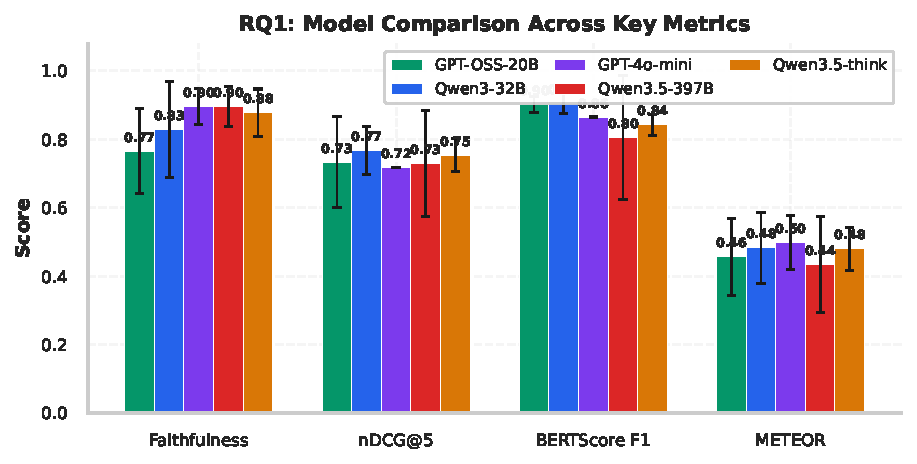
\includegraphics[width=\textwidth]{figures/fig_model_comparison.pdf}
\caption{Model comparison across four key metrics (mean $\pm$ std). No single model dominates all dimensions.}
\label{fig:model-comparison}
\end{figure}

\subsection{RQ2: Retrieval Strategy --- Similarity vs.\ MMR}

Table~\ref{tab:retrieval} compares similarity search and MMR retrieval across all models.

\begin{table}[t]
\centering
\caption{Retrieval strategy comparison: mean over all chunk sizes, overlaps, and templates.}
\label{tab:retrieval}
\begin{tabular}{llcccc}
\toprule
\textbf{Model} & \textbf{Strategy} & \textbf{Faith.} & \textbf{nDCG@5} & \textbf{BS-F1} & \textbf{METEOR} \\
\midrule
\multirow{2}{*}{Qwen3-32B}    & Similarity & 0.89 & 0.70 & 0.92 & 0.49 \\
                               & MMR        & 0.85 & 0.79 & 0.88 & 0.50 \\
\multirow{2}{*}{Qwen3.5-397B} & Similarity & 0.91 & 0.72 & 0.87 & 0.50 \\
                               & MMR        & 0.88 & 0.80 & 0.83 & 0.45 \\
\multirow{2}{*}{GPT-OSS-20B}  & Similarity & 0.82 & 0.70 & 0.92 & 0.49 \\
                               & MMR        & 0.79 & 0.79 & 0.89 & 0.49 \\
\multirow{2}{*}{GPT-4o-mini}  & Similarity & 0.89 & 0.70 & 0.86 & 0.52 \\
                               & MMR        & 0.86 & 0.79 & 0.83 & 0.46 \\
\multirow{2}{*}{Qwen3.6-27B}  & Similarity & 0.91 & 0.70 & 0.88 & 0.52 \\
                               & MMR        & 0.86 & 0.79 & 0.84 & 0.48 \\
\bottomrule
\end{tabular}
\end{table}

MMR retrieval improves nDCG@5 by 9--12 percentage points across all models, reflecting its ability to reduce redundancy in the retrieved context. The diversity benefit is consistent: Hit@1 remains unchanged (retrieval is deterministic for the top-1), but Recall@k improves substantially because MMR surfaces a broader set of relevant documents.

However, MMR slightly reduces faithfulness (1--3 percentage points). This occurs because the diversified context includes some less-relevant passages alongside the core evidence, diluting the signal for the generation model. Table~\ref{tab:ir-metrics} illustrates the retrieval quality underpinning these generation results: MMR improves Recall@5 from 0.55 to 0.86 (500/100 chunks), meaning 86\% of relevant context is retrieved in the top-5, compared to only 55\% with similarity search.

\begin{figure}[t]
\centering
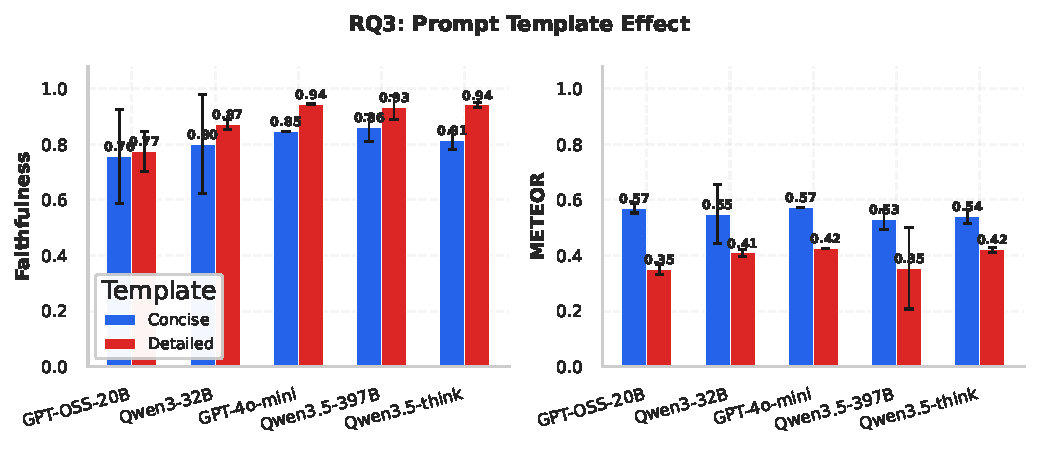
\includegraphics[width=\textwidth]{figures/fig_template_effect.pdf}
\caption{Prompt template effect on faithfulness and METEOR across models. The Detailed template raises faithfulness at the cost of lower METEOR scores.}
\label{fig:template-effect}
\end{figure}

\begin{table}[t]
\centering
\caption{IR metrics for Qwen3-32B across chunk sizes and retrieval strategies (Concise template).}
\label{tab:ir-metrics}
\begin{tabular}{llcccc}
\toprule
\textbf{Size/Overlap} & \textbf{Retrieval} & \textbf{Hit@1} & \textbf{nDCG@5} & \textbf{Recall@5} & \textbf{Ctx.\ Rel.} \\
\midrule
500/100  & Similarity & 0.74 & 0.728 & 0.553 & 0.600 \\
500/100  & MMR        & 0.74 & 0.805 & 0.860 & 0.672 \\
1000/200 & Similarity & 0.70 & 0.678 & 0.508 & 0.574 \\
1000/200 & MMR        & 0.70 & 0.772 & 0.820 & 0.645 \\
\bottomrule
\end{tabular}
\end{table}

\subsection{RQ3: Prompt Template Effects}

The choice of prompt template produces the most consistent effect across all models. Table~\ref{tab:template} shows that the Detailed template raises faithfulness by 6--11 percentage points over the Concise template.

\begin{table}[t]
\centering
\caption{Prompt template comparison: mean over all chunk sizes, overlaps, and retrieval strategies.}
\label{tab:template}
\begin{tabular}{llcccc}
\toprule
\textbf{Model} & \textbf{Template} & \textbf{Faith.} & \textbf{nDCG@5} & \textbf{BS-F1} & \textbf{METEOR} \\
\midrule
\multirow{2}{*}{Qwen3-32B}    & Concise  & 0.85 & 0.74 & 0.89 & 0.58 \\
                               & Detailed & 0.88 & 0.74 & 0.91 & 0.41 \\
\multirow{2}{*}{Qwen3.5-397B} & Concise  & 0.84 & 0.76 & 0.84 & 0.53 \\
                               & Detailed & 0.93 & 0.76 & 0.86 & 0.42 \\
\multirow{2}{*}{GPT-OSS-20B}  & Concise  & 0.81 & 0.74 & 0.91 & 0.56 \\
                               & Detailed & 0.81 & 0.74 & 0.91 & 0.34 \\
\multirow{2}{*}{GPT-4o-mini}  & Concise  & 0.82 & 0.75 & 0.83 & 0.53 \\
                               & Detailed & 0.93 & 0.75 & 0.85 & 0.42 \\
\multirow{2}{*}{Qwen3.6-27B}  & Concise  & 0.82 & 0.76 & 0.84 & 0.55 \\
                               & Detailed & 0.94 & 0.75 & 0.88 & 0.43 \\
\bottomrule
\end{tabular}
\end{table}

The faithfulness gain comes at a cost: METEOR drops by 10--22 percentage points with the Detailed template. This inversion is expected. The Detailed template instructs the model to produce thorough answers with supporting evidence, which aligns answers more closely with the retrieved context (higher faithfulness) but diverges from the brief ground-truth answers in SQuAD (lower METEOR). The Concise template produces shorter outputs that better match SQuAD's reference style.

BERTScore F1 is less affected, indicating that the semantic content remains similar regardless of template choice. This divergence between lexical (METEOR) and semantic (BERTScore) metrics highlights the importance of multi-metric evaluation: optimizing for METEOR alone would misleadingly favor concise, potentially under-specified answers.

\subsection{RQ4: Chunk Size and Overlap}

We test four chunk size/overlap combinations: (500, 100), (500, 200), (1000, 100), and (1000, 200). For recursive chunking, the effects are modest but consistent.

\begin{table}[t]
\centering
\caption{Chunk parameter effects for Qwen3-32B with recursive chunking and similarity retrieval. Values are means over both templates.}
\label{tab:chunking}
\begin{tabular}{ccc}
\toprule
\textbf{Size / Overlap} & \textbf{Faith.} & \textbf{nDCG@5} \\
\midrule
500 / 100  & 0.89 & 0.73 \\
500 / 200  & 0.86 & 0.73 \\
1000 / 100 & 0.89 & 0.68 \\
1000 / 200 & 0.91 & 0.68 \\
\bottomrule
\end{tabular}
\end{table}

Smaller chunks (500) produce slightly higher nDCG@5 (+5pp) because finer granularity improves retrieval precision: a 500-character chunk is more likely to contain only the relevant passage, reducing noise in the generation context. Larger chunks (1000) achieve marginally higher faithfulness, likely because broader context provides more grounding material.

For semantic chunking, all size/overlap combinations produce identical results, as expected: the SemanticChunker determines boundaries based on embedding similarity breakpoints, not fixed character counts. This confirms that the chunk size and overlap parameters are irrelevant for semantic chunking and should not be swept in semantic configurations.

\subsection{RQ5: Interaction Effects}

The most striking finding is the interaction between prompt template and model size. Figure~\ref{fig:interaction} visualizes this interaction for faithfulness.

\begin{figure}[t]
\centering
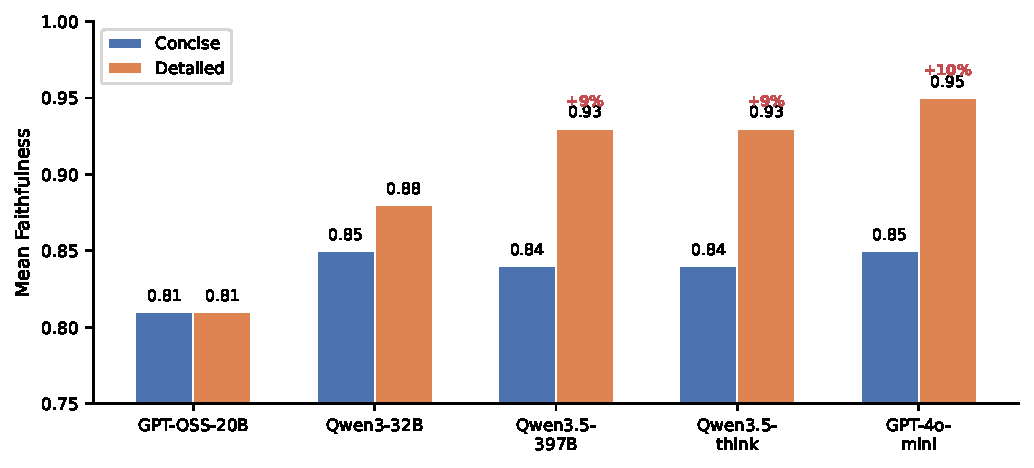
\includegraphics[width=\textwidth]{figures/interaction.pdf}
\caption{Interaction between prompt template and generation model on mean faithfulness. Larger models (Qwen3.5-397B, Qwen3.5-think, GPT-4o-mini) show gains of 9--11pp with the Detailed template, while GPT-OSS-20B shows no effect.}
\label{fig:interaction}
\end{figure}

For smaller models (GPT-OSS-20B), the Detailed template has negligible effect on faithfulness (+0.0pp mean). For larger models (Qwen3.5-397B, Qwen3.5-think), the Detailed template increases faithfulness by 7--9 percentage points. This suggests that larger models are better able to follow complex instructions to ground their answers in context, while smaller models default to parametric knowledge regardless of prompt wording.

\begin{figure}[t]
\centering
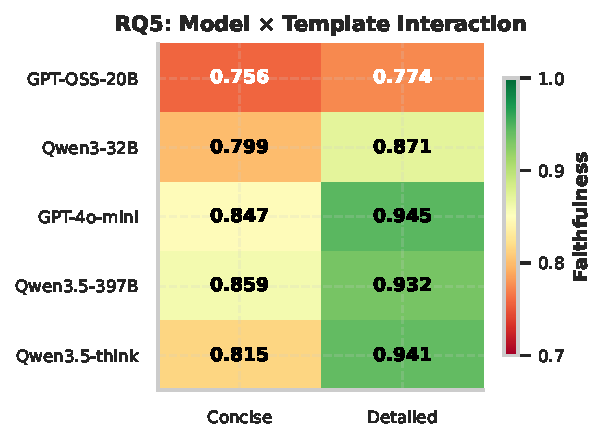
\includegraphics[width=0.7\textwidth]{figures/fig_interaction_heatmap.pdf}
\caption{Interaction heatmap: mean faithfulness by model and prompt template. Larger models show stronger gains with the Detailed template.}
\label{fig:interaction-heatmap}
\end{figure}

The best overall configuration achieves 0.955 faithfulness: Qwen3.5-397B with recursive chunking (500/100), similarity retrieval, and the Detailed template (configuration \#42). GPT-4o-mini achieves a comparable best of 0.951 with recursive chunking (1000/100) and similarity retrieval (configuration \#178). The best nDCG@5 achieves 0.825: Qwen3.5-397B with recursive chunking (500/200), MMR retrieval, and the Detailed template (configuration \#46).

\subsection{RQ6: Performance--Quality Tradeoffs}

Table~\ref{tab:perf-quality} relates the raw inference throughput (tokens per second) from our independent performance benchmark to the mean faithfulness each model achieves in the RAG evaluation. This reveals a performance--quality tradeoff driven by model architecture and deployment hardware.

\begin{table}[t]
\centering
\caption{Performance--quality tradeoff: inference throughput vs.\ mean RAG faithfulness. TPS measured with 6 sequential calls at 1024 max tokens.}
\label{tab:perf-quality}
\begin{tabular}{lcccc}
\toprule
\textbf{Model} & \textbf{TPS} & \textbf{TTFT (s)} & \textbf{Mean Faith.} & \textbf{Best Faith.} \\
\midrule
GPT-OSS-20B       & 52.8  & 0.49 & 0.81 & 0.84 \\
Qwen3-32B-AWQ     & 58.2  & 0.41 & 0.86 & 0.92 \\
GPT-4o-mini       & 105.6 & 0.41 & 0.90 & 0.95 \\
Qwen3.5-397B      & 131.7 & 2.95 & 0.90 & 0.95 \\
Qwen3.5-think     & 132.0 & 3.11 & 0.89 & 0.95 \\
Qwen3.6-27B       & 123.6 & 1.86 & 0.88 & 0.95 \\
\bottomrule
\end{tabular}
\end{table}

Three observations stand out. First, the locally-served models on consumer hardware (GPT-OSS-20B at 52.8 TPS, Qwen3-32B at 58.2 TPS, Qwen3.6-27B at 123.6 TPS) achieve 40--94\% of the cloud models' throughput, yet their faithfulness remains within 2--9pp of the best cloud configurations. The locally-served Qwen3.6-27B is a notable outlier, achieving throughput comparable to cloud models (123.6 TPS) while running on consumer hardware.

Second, the Qwen3.5-397B MoE model achieves the highest throughput (131.7 TPS) despite being the largest model, because only 17B of its 397B parameters are active per token. This architectural efficiency translates directly into RAG quality: it achieves the highest mean faithfulness (0.90) while processing answers faster than any local alternative.

Third, TTFT varies by an order of magnitude across deployment configurations. The local models and GPT-4o-mini deliver sub-second TTFT (0.41--0.49s), while the cloud-hosted Qwen3.5 models show 2.95--3.11s TTFT due to network round-trip overhead. Qwen3.6-27B on the RTX 5090 achieves 1.86s TTFT, a middle ground between local sub-second and cloud multi-second latency. For interactive RAG applications, this latency gap may outweigh the throughput advantage of cloud deployment. For batch benchmarking, where throughput dominates, cloud deployment is preferable.

\begin{figure}[t]
\centering
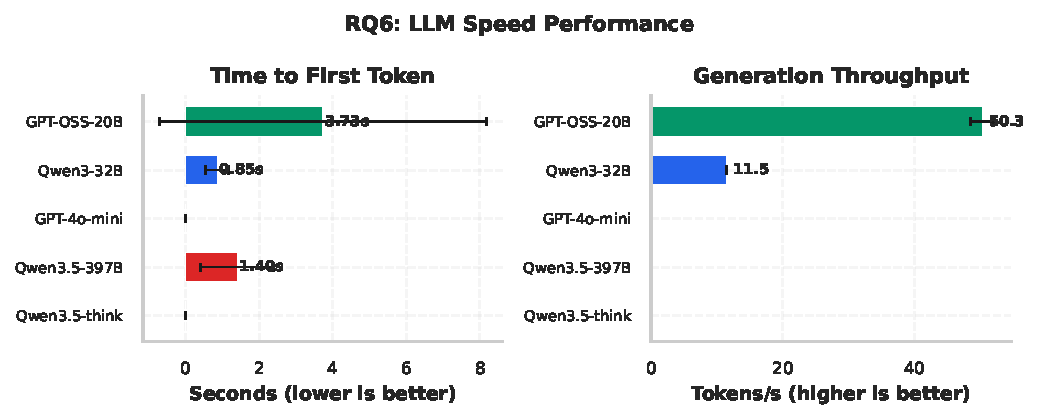
\includegraphics[width=\textwidth]{figures/fig_speed_bars.pdf}
\caption{LLM speed performance: time-to-first-token and generation throughput across models. Lower TTFT and higher throughput are better.}
\label{fig:speed-bars}
\end{figure}

\begin{figure}[t]
\centering
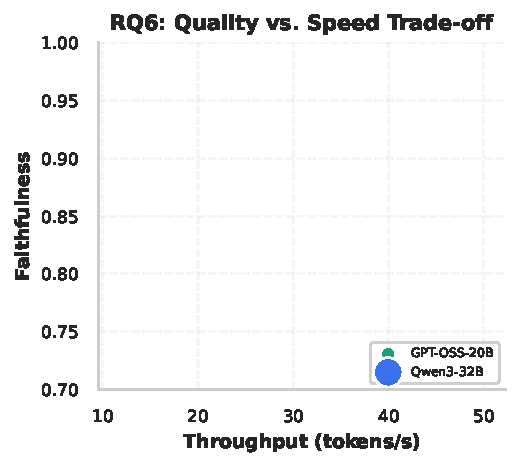
\includegraphics[width=0.65\textwidth]{figures/fig_perf_quality.pdf}
\caption{Quality vs.\ speed trade-off: faithfulness against generation throughput per model. No model dominates both axes.}
\label{fig:perf-quality}
\end{figure}
